
\documentclass[border=8pt, multi, tikz]{standalone} 
\usepackage{import}
\subimport{../layers/}{init}
\usetikzlibrary{positioning}
\usetikzlibrary{3d} %for including external image 

\def\ConvColor{rgb:yellow,5;red,2.5;white,5}
\def\ConvReluColor{rgb:yellow,5;red,5;white,5}
\def\PoolColor{rgb:red,1;black,0.3}
\def\UnpoolColor{rgb:blue,2;green,1;black,0.3}
\def\FcColor{rgb:blue,5;red,2.5;white,5}
\def\FcReluColor{rgb:blue,5;red,5;white,4}
\def\SoftmaxColor{rgb:magenta,5;black,7}   

\newcommand{\copymidarrow}{\tikz \draw[-Stealth,line width=0.8mm,draw={rgb:blue,4;red,1;green,1;black,3}] (-0.3,0) -- ++(0.3,0);}

\begin{document}
\begin{tikzpicture}
\tikzstyle{connection}=[ultra thick,every node/.style={sloped,allow upside down},draw=\edgecolor,opacity=0.7]
\tikzstyle{copyconnection}=[ultra thick,every node/.style={sloped,allow upside down},draw={rgb:blue,4;red,1;green,1;black,3},opacity=0.7]

\node[canvas is zy plane at x=0] (temp) at (-3,0,0) {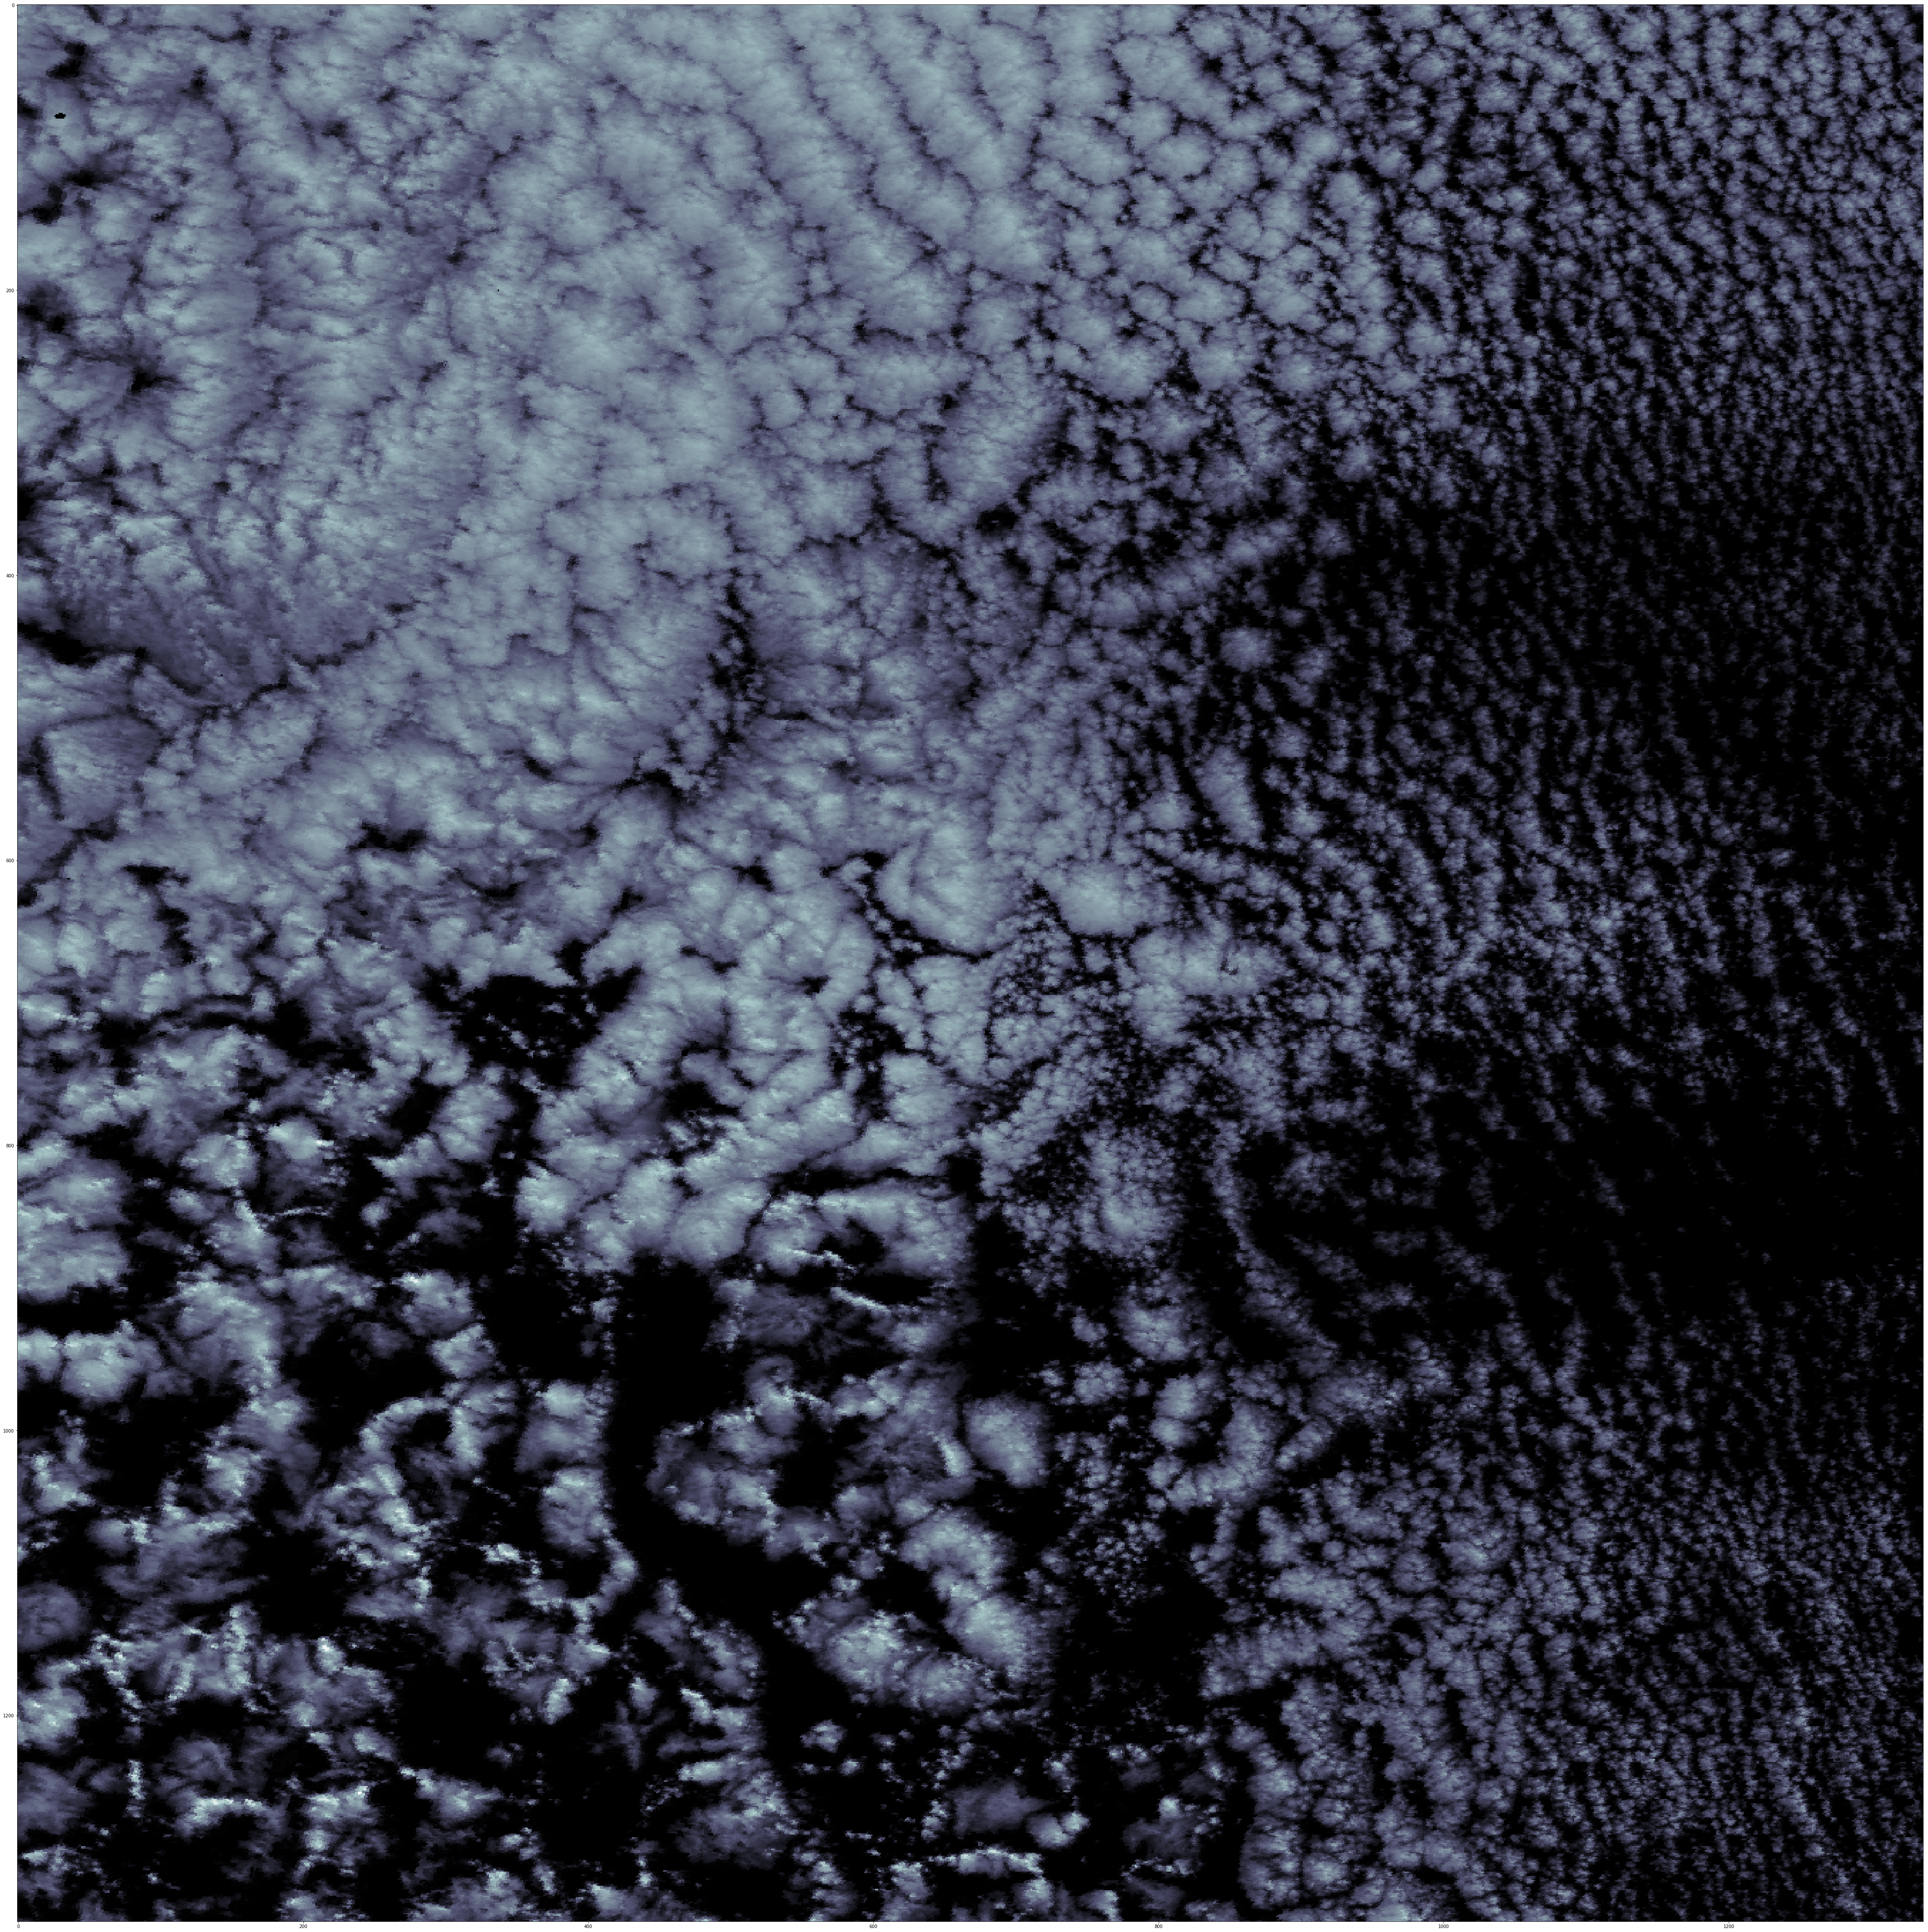
\includegraphics[width=8cm,height=8cm]{./coast_of_chile_high_res.png}};

% \pic[shift={(0,0,0)}] at (0,0,0) 
%     {Box={
%         name=testconv,
%         caption=TESTE,
%         xlabel={{64, }},
%         zlabel=500,
%         fill=\ConvColor,
%         height=50,
%         width=(2, 2),
%         depth=50
%         }
%     };

\pic[shift={ (0,0,0) }] at (0,0,0) 
    {RightBandedBox={
        name=ccr_b1,
        caption=,
        xlabel={{ 64, 64 }},
        zlabel=500,
        fill=\ConvColor,
        bandfill=\ConvReluColor,
        height=40,
        width={ 2 , 2 },
        depth=40
        }
    };

\pic[shift={ (0,0,0) }] at (ccr_b1-east) 
    {Box={
        name=pool_b1,
        caption= ,
        fill=\PoolColor,
        opacity=0.5,
        height=32,
        width=1,
        depth=32
        }
    };

\pic[shift={ (1,0,0) }] at (pool_b1-east) 
    {RightBandedBox={
        name=ccr_b2,
        caption= ,
        xlabel={{ 128, 128 }},
        zlabel=256,
        fill=\ConvColor,
        bandfill=\ConvReluColor,
        height=32,
        width={ 3.5 , 3.5 },
        depth=32
        }
    };

\pic[shift={ (0,0,0) }] at (ccr_b2-east) 
    {Box={
        name=pool_b2,
        caption= ,
        fill=\PoolColor,
        opacity=0.5,
        height=24,
        width=1,
        depth=24
        }
    };

\draw [connection]  (pool_b1-east)    -- node {\midarrow} (ccr_b2-west);

\pic[shift={ (1,0,0) }] at (pool_b2-east) 
    {RightBandedBox={
        name=ccr_b3,
        caption= ,
        xlabel={{ 256, 256 }},
        zlabel=128,
        fill=\ConvColor,
        bandfill=\ConvReluColor,
        height=25,
        width={ 4.5 , 4.5 },
        depth=25
        }
    };

\pic[shift={ (0,0,0) }] at (ccr_b3-east) 
    {Box={
        name=pool_b3,
        caption= ,
        fill=\PoolColor,
        opacity=0.5,
        height=19,
        width=1,
        depth=19
        }
    };

\draw [connection]  (pool_b2-east)    -- node {\midarrow} (ccr_b3-west);

\pic[shift={ (1,0,0) }] at (pool_b3-east) 
    {RightBandedBox={
        name=ccr_b4,
        caption= ,
        xlabel={{ 512, 512 }},
        zlabel=64,
        fill=\ConvColor,
        bandfill=\ConvReluColor,
        height=16,
        width={ 5.5 , 5.5 },
        depth=16
        }
    };

\pic[shift={ (0,0,0) }] at (ccr_b4-east) 
    {Box={
        name=pool_b4,
        caption= ,
        fill=\PoolColor,
        opacity=0.5,
        height=12,
        width=1,
        depth=12
        }
    };

\draw [connection]  (pool_b3-east)    -- node {\midarrow} (ccr_b4-west);

\pic[shift={ (2,0,0) }] at (pool_b4-east) 
    {RightBandedBox={
        name=ccr_b5,
        caption=Bottleneck,
        xlabel={{ 1024, 1024 }},
        zlabel=32,
        fill=\ConvColor,
        bandfill=\ConvReluColor,
        height=8,
        width={ 8 , 8 },
        depth=8
        }
    };

\draw [connection]  (pool_b4-east)    -- node {\midarrow} (ccr_b5-west);

\end{tikzpicture}
\end{document}
